Consider the optimization problem $\max x_1 + x_2$, where ($x_1$,
$x_2$) is constrained to belong to the polyhedron represented in Figure \ref{fig:q18-feasible0}.

\begin{figure}[htb]
	\begin{center}
		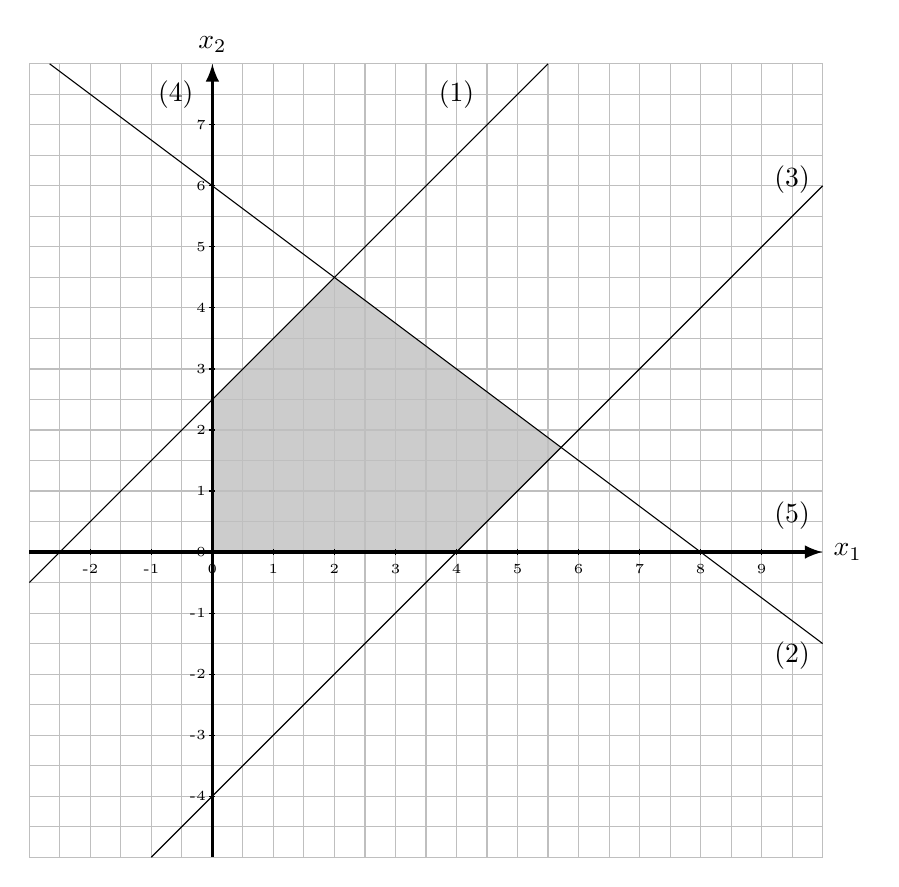
\begin{tikzpicture}[scale=0.775]
		\fill[gray,opacity=0.4] (0,0) -- (0,2.5) -- (2,4.5) -- (40/7,12/7)--(4,0)  --cycle; 
		\draw[gray!50, thin, step=0.5] (-3,-5) grid (10,8);
    	\draw[very thick,-latex] (-3,0) coordinate(x1) -- (10,0) coordinate(x2) node[right] {$x_1$};
    	\draw[very thick,-latex] (0,-5) coordinate(y1) -- (0,8) coordinate(y2) node[above] {$x_2$};
	    \foreach \x in {-2,...,9} \draw (\x,0.05) -- (\x,-0.05) node[below] {\tiny\x};
	    \foreach \y in {-4,...,7} \draw (-0.05,\y) -- (0.05,\y) node[left] {\tiny\y};
	

	    \draw (-3,-0.5)--(5.5,8);
	    \draw (-8/3,8)--(10,-1.5);
%	    \draw (-2,8)--(4.5,-5);
	    \draw (-1,-5)--(10,6);



		\node at (9.5,-1.7){(2)};
		\node at (9.5, 6.1){(3)};
	     \node at (-0.6,7.5){(4)};
	     \node at (9.5,0.6){(5)};
	     \node at (4,7.5){(1)};

	
		
		
		\end{tikzpicture}
		\caption{\label{fig:q18-feasible0}Feasible Domain}
	\end{center}
\end{figure}

\begin{enumerate}
\item Formulate the 5 constraints that determine the feasible domain represented in gray in Figure \ref{fig:q18-feasible0}. 

\item Write the corresponding linear optimization problem in standard form. 

 Give explicitly  the matrix $A$ and the vectors $b$ and $c$.


\item List all  basic solutions of the problem. For each basic solution:
\begin{itemize}
\item   identify the solution on Figure \ref{fig:q18-feasible0},
\item  determine if the solution is feasible.
\end{itemize}

\item Why does point  $(3,$ $2)$ represent a feasible solution, but not a basic solution?

\item Is the direction $d=  \begin{pmatrix}
1 \\
1 
\end{pmatrix}$ feasible for the given feasible point $x= \begin{pmatrix}
4 \\
0 
\end{pmatrix}$? Justify.
\end{enumerate}

